\chapter{Marco Te\'{o}rico}
\label{ch:marco}
%\section{Arquitecturas de Computadoras}

%En concreto, una arquitectura de computadora nos ayuda a especificar los est\'{a}ndares de tecnolog\'{i}a se usaran con respecto al software y de hardware de una computadora. Esto quiere decir que una arquitectura ayuda a establecer el dise\~no de una computadora y las tecnolog\'{a}s con las que este es compatible. Cualquier persona que se dedique a dise\~nar una arquitectura, debe estar consiente de que debe crear un dise\~no l\'{o}gico capaz de satisfacer cualquiera de las necesidades que presente un usuario o un sistema.

%La tarea de un dise\~nador es compleja. Este debe poder determinar los atributos elementales con los que debe contar su dise\~no con el fin de maximizar el desempe\~no y asegurarse que el gasto energ\'{i}a sea de forma eficiente cumpliendo siempre con las restricciones de costo, poder y disponibilidad.

%Dentro de las diversas tareas de un dise\~nador de arquitecturas de computadora, encontramos dos principales: el dise\~no del conjunto de instrucciones y la implementaci\'{o}n \cite{hennessy2011computer}. 

%\subsection{Conjunto de Instrucciones}

%El conjunto de instrucciones o ISA (por sus siglas en ingl\'{e}s, “Instruction Set Architecture") es un grupo de reglas con las cuales el software y el hardware se comunican entre s\'{i}. Estas reglas describen las operaciones, los estados y las localidades que soporta el hardware.

%Existen diversos modelos de ISA, entre los m\'{a}s conocidos, podemos encontrar: CISC (por sus siglas en ingl\'{e}s “Complex Instruction Set Computing") que como su nombre lo indica, permite realizar operaciones muy complejas y se caracterizan por que cada instrucci\'{o}n cuenta con una gran longitud. RISC es otro modelo (“Reduce Instruction Set Computing") el cual cuenta con instrucciones de tama\~no fijo y un reducido n\'{u}mero de formatos, el objetivo de este modelo es propiciar la segmentaci\'{o}n y el paralelismo.


%\subsection{Arquitectura Von Neumann}

%Adem\'{a}s de ISA la implementaci\'{o}n de los componentes representa un papel muy importante. Dentro de las principales arquitecturas, encontramos la de \emph{Von Neumann}. Esta arquitectura se describe por primera vez en 1945 en el reporte escrito por Von Neumann \cite{von1993first}. Los sistemas con microprocesadores se basan en esta arquitectura, en la cual la unidad central de proceso (CPU), está conectada a una memoria principal única donde se guardan las instrucciones del programa y los datos. A dicha memoria se accede a través de un sistema de buses único

%\subsection{Arquitectura Harvard}

 %Por otro lado, contamos con la arquitectura Harvard. El término proviene de la computadora \emph{Harvard mark I}, que almacenaba las instrucciones en cintas perforadas y los datos en interruptores. Esta computadora fue el primer ordenador electromecánico construido en la Universidad Harvard por Howard H. Mark en 1944. En esta arquitectura se utilizan dispositivos separados para las instrucciones y los datos. Para  que haya mayor rapidez se utiliza la memoria cache dividida.
 
 %Como se puede notar, dentro de la arquitectura de von Neumann, el procesador se puede encontrar leyendo una instrucción o escribiendo datos desde o hacia la memoria pero ambos procesos no pueden ocurrir al mismo tiempo ya que las instrucciones y datos usan el mismo sistema de buses. En una computadora que utiliza la arquitectura Harvard, el procesador puede tanto leer una instrucción como realizar un acceso a la memoria de datos al mismo tiempo.

\section{Inteligencia Artificial}

La Inteligencia Artificial (IA) como disciplina formal  ha sido estudiada por más de 50 años. En sus inicios, uno de los principales objetivos de esta disciplina era determinar si una computadora era capaz de “pensar", esta pregunta es igualmente abordada por Alan Turing\cite{turing1950computing} en su obra \emph{Computing Machinery and Intelligence}. La Inteligencia Artificial de manera simple puede ser definida como: el estudio de procesos mentales o intelectuales en t\'{e}rminos de procesos computacionales \cite{aimodern}. Sin embargo, esta definici\'{o}n varia dentro de la literatura \cite{haugeland1985,bellman1978,winston1992learning}. 

Como se puede apreciar, la Inteligencia Artificial tiene una relaci\'{o}n intr\'{i}nseca con la Psicolog\'{i}a, las Ciencias Cognitivas y, a su vez, con las Ciencias en Computaci\'{o}n. Sin embargo, la Inteligencia Artificial no es Psicolog\'{i}a, la distinci\'{o}n recae en que una de las mayores preocupaciones de la Inteligencia Artificial es comprehender de qu\'{e} manera es posible otorgarle a las computadoras una capacidad tan sofisticada como lo es actuar de forma “inteligente".

Adicionalmente, podemos decir que la Inteligencia Artificial intenta entender y crear \emph{agentes inteligentes} capaces de pensar racionalmente. Se enfoca en la inteligencia a trav\'{e}s del pensamiento y la raz\'{o}n. Si este es el caso, se tiene que poder determinar c\'{o}mo los seres humanos piensan. Se necesita indagar en el funcionamiento de las mentes humanas \cite{brooks1995intelligence}.

Actuar racionalmente significa desempe\~nar alguna actividad para alcanzar los objetivos, con base en las creencias de una persona. Un agente es simplemente algo que percibe y actúa. En este enfoque, la IA es vista como el estudio y construcción de agentes racionales \cite{aimodern}.

La IA es un componente base de las ciencias en computaci\'{o}n debido a su abstracción, programación y formalismos lógicos. La IA  desarrolla  herramientas conceptuales para poder comprender c\'{o}mo se procesa la información y estas herramientas son indispensable para que la psicología pueda entender cómo la información es procesada por los seres humanos \cite{nilsson2014principles}.

El campo interdisciplinario de ciencia cognitiva reúne modelos informáticos de IA y técnicas experimentales de
psicología para tratar de construir teorías precisas y comprobables del funcionamiento de la mente humana.

\section{C\'{o}mputo Cognitivo}

A lo largo del la vida, los seres humanos, observan, perciben y reflexionan sobre el medio ambiente y el mundo que los rodea. Reciben informaci\'{o}n del mundo a trav\'{e}s de sus acciones, experiencias y sentidos. De tal forma, que para poder internalizar toda esta informaci\'{o}n, es l\'{o}gico pensar que la comunicaci\'{o}n es difusa, ambigua, esencial para expresar nuestras experiencias \cite{langley2006intelligent}. 

Hoy en día, los humanos crean sistemas virtuales que emulan e interact\'{u}an con nuestro medio ambiente físico. El prop\'{o}sito de estos sistemas, es lograr que interact\'{u}en de forma din\'{a}mica y aut\'{o}noma, que razonen, act\'{u}en y se comuniquen de manera similar a como lo hacen los seres humanos. El principal objetivo del C\'{o}mputo Cognitivo es crear sistemas complejos que imiten los procesos de cognici\'{o}n que llevan a cabo los humanos \cite{crowder2014artificial}.

En general, se entiende a la mente como una colección de procesos de sensaci\'{o}n, percepci\'{o}n, acci\'{o}n, emoci\'{o}n y cognici\'{o}n. La Computaci\'{o}n Cognitiva se enfoca a desarrollar un enfoque coherente, mecanismo unificado y universal con base en las capacidades de la mente. El argumento principal del C\'{o}mputo Cognitivo es que las neur\'{o}nas y las sin\'{a}psis pueden ser descritas por modelos matem\'{a}ticos relativamente compactos, funcionales y fenomenol\'{o}gicos \cite{cc}.

La motivación primordial del C\'{o}mputo C\'{ognitivo} es el hecho de que el comportamiento
del cerebro aparentemente ser rige de manera no aleatoria, con interacciones entre unidades funcionales individuales de control. Esto describe la formaci\'{o}n de sistemas complejos, los cuales, cabe la posibilidad de ser modelados por computadora y simulados para su an\'{a}lisis \cite{cc}

Inteligencia cognitiva real tiene varias manifestaciones, incluyendo la capacidad de adaptarse a situaciones desconocidas en entornos cambiantes din\'{a}micamente.
\section{Arquitecturas Cognitivas}

Como se ha mencionado repetidamente en los p\'{a}rrafos anteriores, un objetivo de la IA consiste en crear agentes racionales capaces de superar el nivel de competencia ante los humanos. A lo largo de los a\~nos se ha observado un gran avance en diferentes \'{a}reas en d\'{o}nde la IA supera a la mente humana: reconocimiento de patrones, memorizaci\'{o}n, recuperaci\'{o}n de grandes vol\'{u}menes de informaci\'{o}n, interpretaci\'{o}n de se\~nales, entre otros. No obstante, cuando se hablan de funciones de cognici\'{o}n de bajo nivel como el reconocimiento de objetos, la IA se encuentra por debajo del desempe\~no de su contraparte natural, la mente humana. Adicionalmente, funciones cognitivas de nivel superior como el lenguaje, el razonamiento, la resoluci\'{o}n de problemas o la planificaci\'{o}n involucran estructuras del conocimiento complejas y son considerablemente m\'{a}s dif\'{i}cil de implementar. 

Si hacemos una comparaci\'{o}n podemos observar que los diferentes tipos de memoria que almacenan informaci\'{o}n en el cerebro facilitan el reconocimiento, asociaci\'{o}n sem\'{a}ntica, interpretaci\'{o}n y recuperaci\'{o}n de un gran n\'{u}mero de patrones de informaci\'{o}n complejos. Por otro lado, la organizaci\'{o}n, almacenamiento y recuperaci\'{o}n de informaci\'{o}n en las computadores es completamente diferente. Las arquitecturas de computaci\'{o}n solo aparentan ser universales, en la pr\'{a}ctica siempre se limita el procesamiento de informaci\'{o}n de manera espec\'{i}fica \cite{duch2008cognitive}. 

Una Arquitectura Cognitiva especifica la infraestructura subyacente de un sistema inteligente. En concreto, una arquitectura incluye aquellos aspectos de un agente cognitivo que son constantes a lo largo del tiempo y entre
diferentes dominios de aplicación \cite{langley2009cognitive}.

Las Arquitecturas Cognitivas casi siempre son elaboradas con el prop\'{o}sito de  modelar el rendimiento humano en múltiples tareas con respecto a diferentes situaciones. Como se ha mencionado antes Allen Newell en su libro \cite{newell1994unified} explica que el principal objetivo de construir una arquitectura cognitiva, es poder formular una teor\'{i}a coherente y unificada inspirada en las capacidades de la mente humana. Adicionalmente, proporciona doce criterios para la evaluación de los sistemas cognitivos: conducta adaptativa, comportamiento dinámico, comportamientos flexibles, desarrollo, evolución, el aprendizaje, la integración de conocimientos, amplia base de conocimientos, lenguaje natural, rendimiento en tiempo real, y la realización del cerebro.

Tres propiedades de diseño clave que subyacen en el desarrollo de cualquier arquitectura cognitiva son la memoria,
el aprendizaje y la representaci\'{o}n del conocimiento \cite{langley2009cognitive,duch2008cognitive}. Varios tipos de memoria sirven como depósito para la gran cantidad de informaci\'{o}n, conocimientos y creencias sobre el mundo y de uno mismo; por otro lado, el aprendizaje es el proceso principal que da forma a este conocimiento. La organizaci\'{o}n de la memoria depende de los esquemas de representación del conocimiento. 
 
 No está claro en absoluto si las arquitecturas cognitivas, que se ejecuta en ordenadores convencionales, llegar\'{a}n a la flexibilidad del cerebro en las funciones cognitivas de nivel superior o inferior.
 
 Uno de los primeros intentos en crear una arquitectura cognitiva se refleja en \emph{SOAR}. Se inici\'{o} el desarrollo de este marco de trabajo desde los inicios de la investigaci\'{o}n sobre el c\'{o}mputo cognitivo. Sin embargo, no es la \'{u}nica arquitectura existente, pero s\'{i} una de las m\'{a}s utilizadas y conocidas.

\section{SOAR}

\emph{SOAR} (por sus siglas en ingl\'{e}s: “State, Operator And Result") es una arquitectura para poder construir un sistema que sea capaz de ejecutar inteligencia general. \emph{SOAR} cuenta con la capacidad de: primero, trabajar en una amplia gama de tareas, desde problemas rutinarios hasta extremadamente dif\'{i}ciles; segundo, utiliza una gran diversidad de m\'{e}todos para la resoluci\'{o}n de problemas e implementa representaciones adecuadas para dichos problemas; por \'{u}ltimo aprende sobre las caracter\'{i}sticas de los problemas que soluciona y analiza cu\'{a}l fue su propio desempe\~no dentro de las diferentes tareas.

 \emph{SOAR} es uno de los muchos sistemas de IA que han intentado proporcionar una organizaci\'{o}n apropiada con capacidades similares a un agente inteligente y racional. Esta arquitectura tiene su raíces con la aparición del concepto de arquitectura cognitiva \cite{newell1973production}.
 %RECUERDA CAMIAR LOS SIGUIENTES PARRAFOS PORQUE YA ES COPY PASTE
 \emph{SOAR} ha estado en continuo desarrollo desde principios de 1980. 
 
 El conocimiento procedimental a largo plazo en esta arquitectura toma la forma de reglas de producción, que son a su vez organizada en t\'{e}rminos de los operadores asociados con espacios de los problemas. Algunos operadores describen acciones simples, primitivas que modifican el estado interno del agente o generan acciones externas primitivas. Durante muchos años, \emph{SOAR} a utilizado el modelo anteriormente mencionado para representar el conocimiento a largo plazo. Recientemente, se han añadido recuerdos epis\'{o}dicos y sem\'{a}nticos diferentes. La memoria epis\'{o}dica  mantiene un historial de estados anteriores, mientras que la memoria sem\'{a}ntica contiene hechos conocidos previamente\cite{laird1987soar}.
 
Todas las tareas en \emph{SOAR} se formulan como intentos de lograr objetivos. Los operadores realizan los b\'{a}sicos actos deliberativos del sistema, con conocimientos utilizados para determinar din\'{a}micamente su selección y solicitud. El ciclo de procesamiento b\'{a}sico propone repetidamente, selecciona y aplica operadores de la
espacio del problema actual a un estado de problema siguiente, avanzando una decisi\'{o}n a la vez. Sin embargo, cuando el conocimiento acerca de la selección del operador es insuficiente para determinar el siguiente operador  o cuando un operador abstracto no puede ser implementado, un callejón sin salida se produce; en respuesta, \emph{SOAR} crea un nuevo objetivo para determinar qué operador debe seleccionar o c\'{o}mo se debe aplicar el operador abstracto\cite{langley2009cognitive}.

Dentro de las capacidades de \emph{SOAR} podemos encontrar:

\begin{itemize}
  \item trabajar con una amplia gama de tareas, como se espera de un agente inteligente,
  \item utilizar y representar de manera adecuada el conocimiento,
  \item utilizar m\'{e}todos de resoluci\'{o}n de problemas,
  \item interactuar con el medio ambiente,
  \item aprender sobre su propio desempe\~no en las tareas que realiza 
\end{itemize}


Al igual que los sistemas de resolución de problemas y razonamiento en IA m\'{a}s comunes, SOAR tiene una representaci\'{o}n simb\'{o}lica expl\'{i}cita de sus tareas, que se manipula por procesos simb\'{o}licos. Codifica su conocimiento de la tarea en un ambiente de estructuras simb\'{o}licas e intenta utilizar este conocimiento para guiar su comportamiento \cite{laird1987soar}.

\section{Modelos Gr\'{a}ficos}
Un "modelo gráfico" es un tipo de red probabil\'{i}stica que tiene sus ra\'{i}ces en varias comunidades de investigaci\'{o}n diferentes, incluyendo la inteligencia artificial, estadísticas y redes neuronales. El marco de trabajo de los modelos gr\'{a}ficos proporciona un formalismo mate\'{a}tico sencillo y unificado que ha hecho posible entender las relaciones entre una amplia variedad de enfoques con base en redes.

Los modelos gr\'{a}ficos utilizan grafos para representar y manipular distribuciones de probabilidad conjunta. El grafo subyacente a un modelo gr\'{a}fico puede ser dirigido, en cuyo caso el modelo es frecuentemente llamado como redes de creencias o redes bayesianas; en el caso de un grafo no dirigido, se le llama campos aleatorios de Markov.
\subsection{Redes Bayesianas}

Las redes bayesianas son una representaci\'{o}n gr\'{a}fica de dependencias para razonamiento probabil\'{i}stico, en la cual los nodos representan variables aleatorias y los arcos representan relaciones de dependencia directa entre las variables \cite{torres1998bayesian}. Una red bayesiana es un grafo ac\'{i}clico dirigido (al que llamaremos $G$) junto con una distribuci\'{o}n de probabilidad particular ($p$).

Una red bayesiana representa en forma gr\'{a}fica las dependencias e independencias entre variables aleatorias, en particular las independencias condicionales. Lo anterior se representa con la siguiente notaci\'{o}n, para el caso de X independiente de Y dado Z: $P(X|Y,Z)=P(X|Z)$

Cada nodo tiene asociado una función de probabilidad que toma como entrada un conjunto particular de valores de las variables padres del nodo y devuelve la probabilidad de la variable representada por el nodo. Por ejemplo, si por padres son $m$ variables booleanas entonces la función de probabilidad puede ser representada por una tabla de $2^m$ entradas, una entrada para cada una de las $2^m$ posibles combinaciones de los padres siendo verdadero o falso.

Siempre es posible representar a una distribuci\'{o}n conjunta como un producto de condicionales de una sola variable. Dado un ordenamiento $X_1,X_2,…,X_k$, podemos escribir (por la regla del producto):

$$p(x_1, \ldots ,x_k)=p(x_1)p(x_2|x_1)p(x_3|x_1,x_2) \cdots p(x_k|x_1,\ldots ,x_{k-1})$$

En primer lugar, una factorizaci\'{o}n de la conjunta puede ser entendida como una parametrizaci\'{o}n particular de la conjunta a trav\'{e}s de sus distribuciones condicionales. En segundo lugar, los grafos dirigidos ac\'{i}clicos asociados a una distribuci\'{o}n conjunta dan una factorizaci\'{o}n particular $p$ para la conjunta \cite{koller2009probabilistic}.

Sea $G$ un grafo dirigido con v\'{e}rtices $X_1,X_2,\ldots,X_k$, denotamos por $Pa(x_i)$ a todos los padres de $X_i$ en $G$.

Sea $p$ una distribuci\'{o}n conjunta para $X_1,X_2,\ldots,X_k$. Decimos que $G$ representa a $p$ cuando la conjunta se factoriza como:
$$p(x_1,x_2,\ldots,x_n)= \Pi^k_{i=1}=p(x_i|Pa(x_i))$$.

El conjunto de distribuciones que son representadas por $G$ lo denotamos por $M(G)$. N\'{o}tese que un grafo ac\'{i}clico no dirigido no establece una distribuci\'{o}n particular, sino un conjunto de posibles distribuciones: todas las distribuciones que se factorizan bajo $G$.
%%%%%CAMBIAR EL EJEMPLO Y LA IMAGEN
\begin{figure}[h]
\caption{Ejemplo de una Red Bayesiana}
\centering
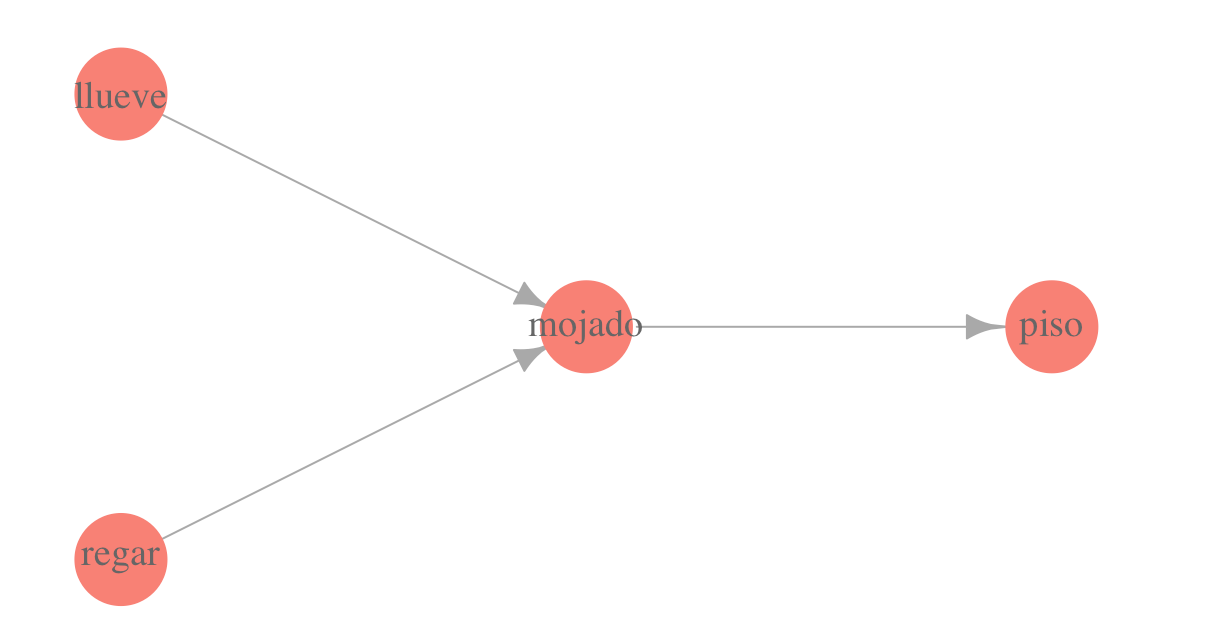
\includegraphics[width=7.0 cm, height = 4.5 cm ]{red.png}
\label{fig:red1}
\end{figure}

Por ejemplo, en la Figura \ref{fig:red1} podemos observar que la conjunta $p(m,l,r,z)$ ($z$ es piso resbaloso) se factoriza como: $p(l)p(r)p(m|l,r)p(z|m)$

\subsection{Modelos Ocultos de Markov}
Un modelo oculto de Markov es una cadena de q junto con un proceso estoc\'{a}stico que
toma valores en un alfabeto $\Sigma$ y el cual depende de $q$.
Estos sistemas evolucionan en el tiempo pasando aleatoriamente de estado a estado y
emitiendo en cada momento al azar algún símbolo del alfabeto $\Sigma$. Cuando se encuentra
en el estado $q_{t-1} = i$, tiene la probabilidad $a
_{ij}$ de moverse al estado $q_t = j$ en el siguiente
instante y la probabilidad $b_j(k)$ de emitir el s\'{i}mbolo $o_t = v_k$ en el tiempo $t$.
S\'{o}lamente los s\'{i}mbolos emitidos por el proceso q son observables, pero no la ruta o
secuencia de estados $q$, de ah\'{i} el calificativo de “oculto" de Markov, ya que el proceso
de Markov $q$ es no observado. 

Consideramos datos secuenciales $X_1,\ldots,X_T$. Un modelo markoviano de estado oculto se factoriza como (es decir, cumple las relaciones de independencia condicional indicadas en el el grafo de la Figura \ref{fig:red2}):

\begin{figure}[h]
\caption{Ejemplo de una cadena oculta de Markov}
\centering
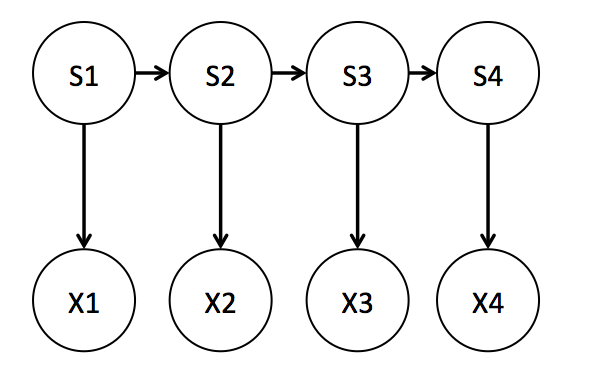
\includegraphics[width=7.0 cm, height = 4.5 cm ]{markov.png}
\label{fig:red2}
\end{figure}

Las variables $S_t$ (estado oculto) son latentes. Las variables $X_t$ no son independientes, pero son condicionalmente independientes dados los estados ocultos. El modelo está dado por una factorizaci\'{o}n que solo incluye t\'{e}rminos de la forma $P(S_t|S_{t-1})$, $P(X_t|S_t)$ y $P(S_1)$. En los modelos de transición de estados suponemos homogeneidad de la cadena de Markov subyacente, es decir,
$P(S_t=j|S_{t-1}=i)=p_{ij}$ no depende de $t$.

En los modelos de respuesta o de observación, las variables observadas $X_t$ pueden ser discretas o continuas. Si $X_t$ son discretas, cada $P(X_t|S_t)$ está dada por una tabla, que tambi\'{e}n suponemos homog\'{e}nea (no depende de $t$). Si $X_t$ son continuas, entonces estas probabilidades est\'{a}n dadas por densidades condicionales.

\subsection{Grafos de Factor}
Este modelo gr\'{a}fico proporciona una forma de “divide y vencer\'{a}s" con
componentes que pueden ser descompuestos para reducir el
combinatoria que surge con funciones de m\'{u}ltiples
variables. La funci\'{o}n podr\'{i}a ser una probabilidad conjunta
distribuci\'{o}n sobre un conjunto de variables aleatorias o un problema que implica la satisfacci\'{o}n de restricciones sobre un conjunto de variables

La operación de gráfico t\'{i}pica es el factor de
c\'{a}lculo de las marginales en las variables. Para una 
distribución de probabilidad conjunta, esto es simplemente el marginal de una
variable aleatoria, que se calcula con la suma de las otras 
variables: $P(Y)= \Sigma_{v,w,x,z}P(v,w,x,Y,z)$

Para las probabilidades,
la distribuci\'{o}n conjunta se descompone en un producto de
condicionales (\emph{prior}) probabilidades sobre subconjuntos de las
variables: $P(V,W,X,Y,Z)=P(V)P(W)P(X|V,W)P(Y|X)P(Z|X)$

Tales descomposiciones derivan de la regla de la cadena y de supuestos de independencia condicional.
